\begin{pa} \label{PA:10.7} The quantity of a product demanded by consumers is often a function of the price of the product. The quantity of demand for a product may also depend on the price of other products (the demand for McDonald's hamburgers may be affected by the price of Burger King hamburgers, or the demand for gas at one station can be affected by the price of gas at another). Suppose quantities demanded $q_1$ and $q_2$ of two goods are dependent on their respective prices $p_1$ and $p_2$ as follows:
\begin{align}
q_1 &= 150 - 2p_1 - p_2 \label{eq:good1} \\
q_2 &= 200 - p_1 - 3p_2. \label{eq:good2}
\end{align}
A problem for the manufacturer and seller of both products is how to set prices in order to maximize revenue.

We assume the maximal revenue will occur when the manufacturer sells all of the products. So if we let $f$ be the revenue obtained by selling $q_1$ items of good one at price $p_1$ per item and $q_2$ items of good two at price $p_2$ per item, then
\[f(p_1, p_2, q_1, q_2) = p_1q_1 + p_2q_2.\]
We can reduce the revenue to a function of just two variables $p_1$ and $p_2$ by using (\ref{eq:good1}) and (\ref{eq:good2}), giving us
\[f(p_1,p_2) = p_1(150 - 2p_1 - p_2) + p_2(200 - p_1 - 3p_2)= 150p_1 + 200p_2 - 2p_1p_2 -2p_1^2 - 3p_2^2.\]
A graph of $f$ as a function of $p_1$ and $p_2$ is shown in Figure \ref{F:Optimize1}.
\begin{figure}[h]
\begin{center}
\resizebox{!}{2.0in}{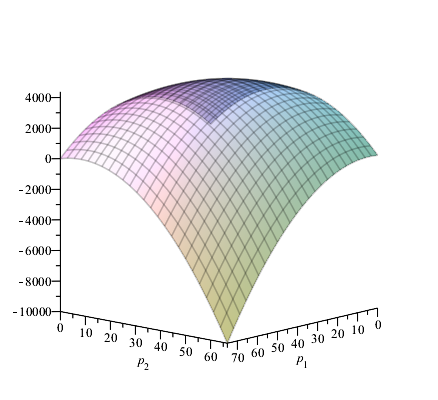
\includegraphics[trim=0cm 0cm 0.5cm 1cm,clip]{10_7_Optimize1}}
\end{center}
\caption{A revenue function.}
\label{F:10.7.Optimize1}
\end{figure}
%crop graphics in animate trim=<left> <bottom> <right> <top>, clip
    \ba
    \item Does it appear that there is a maximum value for the revenue. Why?



\begin{comment}

It looks like the surface in Figure \ref{F:Optimize1} reaches a high point, so it does appear that there is a maximum value for the revenue.



\end{comment}

    \item Based on the graph of the revenue surface in Figure \ref{F:10.7.Optimize1}, describe what you think the tangent plane to the surface looks like at the point where the maximum value occurs. What should we expect the values of $\frac{\partial f}{\partial p_1}$ and $\frac{\partial f}{\partial p_2}$ to be at this maximum value?



\begin{comment}

At the highest point, it looks like the tangent plane is horizontal, and so we should expect $\nabla f$ to be 0. In other words, at the maximum value we should have $\frac{\partial f}{\partial p_1} = 0$ and $\frac{\partial f}{\partial p_2} = 0$.


\end{comment}

    \item Assume your response to part (b) is correct. Use this response to find the maximum revenue.



\begin{comment}

We calculate $\frac{\partial f}{\partial p_1}$ and $\frac{\partial f}{\partial p_2}$ and find out when they are simultaneously 0. Now
\[\frac{\partial f}{\partial p_1} = 150 - 2p_2 - 4p_1 \ \ \text{ and } \ \ \frac{\partial f}{\partial p_2} = 200 - 2p_1 - 6p_2.\]
The system
\begin{align*}
\frac{\partial f}{\partial p_1} &= 0 \\
\frac{\partial f}{\partial p_2} &= 0
\end{align*}
or
\begin{align*}
150 - 2p_2 - 4p_1 &= 0 \\
200 - 2p_1 - 6p_2 &= 0
\end{align*}
is a system of two linear equations in two unknowns. Multiplying both sides of the second equation by $-2$ and then adding corresponding sides of this new equation with the first equation yields the equation
\[-250 + 10p_2 = 0\]
or
\[p_2 = 25.\]
Substituting back into the first equation shows that
\[p_1 = 25.\]
So the maximum revenue occurs with $p_1=p_2 = 25$ and the maximum revenue is
\[f(25,25) = 4375.\]



\end{comment}

    \ea
\end{pa} \afterpa 